% ==========================================================================
% EMPR — 主稿（LaTeX）
%
% 数字规则：本文件**不写任何手抄数字**。
%   - 表格：\input{paper/tableN_*.tex}（由 scripts/make_paper_tables.py 生成）
%   - 行内数字：一律引用 paper/numbers.tex 里的宏（同脚本生成）
% 因此"论文以哪个为准"的答案是：以本文件为准，而本文件的数字全部指向 results/。
% 更新流程：重跑实验 -> python scripts/make_paper_tables.py -> 重新编译本文。
%
% 编译：cd paper && latexmk -pdf main.tex   （详见 paper/BUILD.md）
% ==========================================================================
\documentclass[10pt,letterpaper]{article}

\usepackage[T1]{fontenc}
\usepackage[utf8]{inputenc}
\usepackage{amsmath,amssymb}
\usepackage{booktabs,multirow,array}
\usepackage{graphicx}
\usepackage{xcolor}
\usepackage[margin=1in]{geometry}
\usepackage[hidelinks]{hyperref}
\usepackage[numbers,sort&compress]{natbib}
\usepackage{caption}
\captionsetup{font=small,labelfont=bf}
\usepackage{titlesec}
\titlespacing*{\section}{0pt}{1.2ex plus .3ex}{0.6ex}
\graphicspath{{../results/}{./}}

% 由 scripts/make_paper_tables.py 自动生成，请勿手改。
% 正文里的每个数字都应引用这里的宏，避免与 results/ 不一致。
%
% 关键宏的定义（供人工核对，避免同名不同义）：
%   \nbWordingFlips == \nbRightToWrong + \nbWrongToRight
%       即 cross-the-boundary 的不一致对总数，不是「答案数值改变数」
%   \nbWordingCovered / \nbNumericCovered = 该变体实际覆盖的题数（分母）
%   \acc* = 正确率（百分数，一位小数）；\nb* = 样本量；\pct* = 百分比
%   \chiSameFamily  <- results/error_labels.json（Qwen2.5-14B 同族标注）
%   \chiCrossFamily <- results/error_labels_llama.json（Llama-3.1-8B 异族标注）
%   \plateauLo/Hi   <- 与峰值层不可区分的最大连续层区间（配对 bootstrap 定义）
%   以上均经 results/paper_stats.json 中转，可逐项追溯到原始运行
\providecommand{\nb}[1]{#1}
\newcommand{\accCotThreeB}{12.1}
\newcommand{\accCotSevenB}{21.1}
\newcommand{\accCotFourteenB}{25.7}
\newcommand{\accCotLlamaEightB}{9.9}
\newcommand{\accCotROneSevenB}{11.1}
\newcommand{\accDirThreeB}{5.3}
\newcommand{\accDirSevenB}{8.7}
\newcommand{\accDirFourteenB}{11.8}
\newcommand{\accDirLlamaEightB}{7.7}
\newcommand{\ciCotSevenBLo}{16.7}
\newcommand{\ciCotSevenBHi}{25.7}
\newcommand{\ciCotFourteenBLo}{21.1}
\newcommand{\ciCotFourteenBHi}{30.7}
\newcommand{\ratioSevenB}{2.43}
\newcommand{\ratioFourteenB}{2.18}
\newcommand{\ratioLlamaEightB}{1.29}
\newcommand{\ratioThreeB}{2.28}
\newcommand{\gapFourteenVsSevenCot}{4.6}
\newcommand{\nbSciBench}{323}
\newcommand{\nbOlympiadAll}{351}
\newcommand{\nbOlympiadScorable}{152}
\newcommand{\pctOlympiadScorable}{43}
\newcommand{\nbMMLU}{488}
\newcommand{\accMMLU}{66.6}
\newcommand{\accOlySevenB}{23.7}
\newcommand{\accOlyFourteenB}{30.3}
\newcommand{\gapOlyFourteenVsSeven}{6.6}
\newcommand{\pctChangedThreeBNumeric}{77.0}
\newcommand{\pctChangedThreeBWording}{33.8}
\newcommand{\pctChangedThreeBSwap}{83.3}
\newcommand{\pairBaseThreeB}{5.4}
\newcommand{\pairVarThreeB}{5.4}
\newcommand{\pairDeltaPPThreeB}{0.0}
\newcommand{\pairPThreeB}{0.752}
\newcommand{\pctChangedSevenBNumeric}{77.7}
\newcommand{\pctChangedSevenBWording}{30.4}
\newcommand{\pctChangedSevenBSwap}{69.4}
\newcommand{\pairBaseSevenB}{8.3}
\newcommand{\pairVarSevenB}{9.6}
\newcommand{\pairDeltaPPSevenB}{1.2}
\newcommand{\pairPSevenB}{0.371}
\newcommand{\pctChangedFourteenBNumeric}{83.9}
\newcommand{\pctChangedFourteenBWording}{31.7}
\newcommand{\pctChangedFourteenBSwap}{80.6}
\newcommand{\pairBaseFourteenB}{11.7}
\newcommand{\pairVarFourteenB}{13.8}
\newcommand{\pairDeltaPPFourteenB}{2.1}
\newcommand{\pairPFourteenB}{0.131}
\newcommand{\pctChangedLlamaEightBNumeric}{57.4}
\newcommand{\pctChangedLlamaEightBWording}{24.4}
\newcommand{\pctChangedLlamaEightBSwap}{63.9}
\newcommand{\pairBaseLlamaEightB}{8.3}
\newcommand{\pairVarLlamaEightB}{7.9}
\newcommand{\pairDeltaPPLlamaEightB}{-0.4}
\newcommand{\pairPLlamaEightB}{1.000}
\newcommand{\nbCausalAttempts}{150}
\newcommand{\nbCausalValid}{14}
\newcommand{\nbCausalCleanWrong}{134}
\newcommand{\nbCausalFlat}{2}
\newcommand{\nbLayers}{28}
\newcommand{\nbLayerStep}{2}
\newcommand{\peakLayer}{8}
\newcommand{\peakRecovery}{0.84}
\newcommand{\nbAllAttempts}{100}
\newcommand{\nbCleanCorrect}{10}
\newcommand{\nbCleanWrong}{90}
\newcommand{\pctParseCorrupt}{96}
\newcommand{\pctParseMin}{97}
\newcommand{\pctParseMax}{100}
\newcommand{\pctAccCleanCorrectBest}{70}
\newcommand{\pctAccCleanWrongBest}{3.3}
\newcommand{\kappaAnnotators}{0.133}
\newcommand{\pctAgreeAnnotators}{60}
\newcommand{\nbAnnotated}{495}
\newcommand{\peakCiLo}{0.69}
\newcommand{\peakCiHi}{0.95}
\newcommand{\nbNonseparableLayers}{6}
\newcommand{\plateauLo}{4}
\newcommand{\plateauHi}{14}
\newcommand{\nbPlateauLayers}{6}
\newcommand{\nbBothRight}{19}
\newcommand{\nbRightToWrong}{1}
\newcommand{\nbWrongToRight}{4}
\newcommand{\nbWordingFlips}{5}
\newcommand{\pWordingExact}{0.375}
\newcommand{\chiSameFamily}{4.55}
\newcommand{\pChiSameFamily}{0.208}
\newcommand{\chiCrossFamily}{1.09}
\newcommand{\pChiCrossFamily}{0.778}
\newcommand{\kappaLinearWeighted}{0.118}
\newcommand{\pctAgreeEtwo}{88}
\newcommand{\pctAgreeEone}{16}
\newcommand{\wilsonCcLo}{40}
\newcommand{\wilsonCcHi}{89}
\newcommand{\nbCleanCorrectK}{7}
\newcommand{\wilsonCwLo}{1.1}
\newcommand{\wilsonCwHi}{9.3}
\newcommand{\nbCleanWrongK}{3}
\newcommand{\nbNumericCovered}{305}
\newcommand{\nbWordingCovered}{240}
\newcommand{\nbSwapCovered}{36}
\newcommand{\accScafCot}{24.0}
\newcommand{\pctNoAnswerCot}{71}
\newcommand{\nbScafCot}{150}
\newcommand{\accScafStruct}{26.0}
\newcommand{\pctNoAnswerStruct}{90}
\newcommand{\nbScafStruct}{150}
\newcommand{\scafDeltaPP}{+2.0}
\newcommand{\scafP}{0.700}
\newcommand{\nbTests}{84}
\newcommand{\nbSelfCheck}{23}
\newcommand{\gpuHoursTotal}{2.6}
\newcommand{\nbEvalRuns}{14}
\newcommand{\nbRunsTotal}{25}


\newcommand{\TODO}[1]{\textcolor{red}{[TODO: #1]}}

\title{\textbf{Surface-Conditioned Computation:\\
Probing Whether Open LLMs Compute or Retrieve on Physics Problems}}
\author{Anonymous Authors}
\date{}

\begin{document}
\maketitle

% ---------------------------------------------------------------- Abstract
\begin{abstract}
We ask whether open-weight language models actually \emph{compute} when they
answer multi-step physics problems, or whether they pattern-match against
memorised solutions. Rather than reporting a single accuracy number, we combine
five probes on SciBench physics (\nbSciBench{} problems), a multiple-choice
control (MMLU physics, \nbMMLU{} problems) and a second free-response benchmark
(OlympiadBench physics, \nbOlympiadAll{} problems).
Three findings carry the paper. First, \emph{prompting outweighs scale}:
chain-of-thought multiplies accuracy by \ratioThreeB--\ratioFourteenB$\times$
across the Qwen2.5 family, whereas doubling parameters from 7B to 14B adds only
\gapFourteenVsSevenCot{} points, and the benefit is family-dependent rather than
universal (\ratioLlamaEightB$\times$ for Llama-3.1-8B). Second, \emph{knowledge
is present but execution is not}: the same 7B model answers \accMMLU\% of
multiple-choice physics items but only \accCotSevenB\% when it must produce the
number itself. Third, \emph{answers are surface-conditioned}: a paraphrase that
leaves physics and data bit-identical changes \pctChangedSevenBWording\% of final
answers in every model we test, yet moves only \nbWordingFlips{} of 240 items
across the correct/incorrect boundary, so the instability is value-level wandering
rather than a systematic difficulty change.
Two further probes constrain the mechanism. Corrupt-and-restore causal tracing
localises recoverable behaviour to an early-middle band (roughly layers 4--16 of
\nbLayers) that we can identify as a range but \emph{not} as a single peak layer,
and separating output execution from correctness shows that parseability is
layer-invariant while correctness is not; on problems the model cannot solve,
restoration never rescues them at any single layer. Error annotation
cross-checked by a second, cross-family judge indicates that arithmetic rather
than physical knowledge dominates the failures, but agreement between the judges
is only $\kappa=\kappaAnnotators$, so we claim only annotator-robust statements
and release the dual-annotated sample as a resource for LLM-as-a-judge research.
All experiments ran on a single 80\,GB GPU in about \gpuHoursTotal{} GPU-hours.
\end{abstract}

% ---------------------------------------------------------------- 1 Intro
\section{Introduction}
\label{sec:intro}

Chain-of-thought prompting \citep{wei2022cot} is routinely credited with giving
language models ``reasoning'' ability, and physics benchmarks such as SciBench
\citep{wang2023scibench} and OlympiadBench \citep{he2024olympiadbench} are used to
demonstrate progress. A single accuracy number, however, cannot distinguish two
very different internal situations: a model that derives the answer from the
stated quantities, and a model that recognises the problem family and emits a
plausible-looking number.

\paragraph{A binary framing, deliberately, and how the data refine it.}
We organise the study around the question ``compute or retrieve?'' because it
generates falsifiable predictions: a retrieving model should be insensitive to
the numerical values and highly sensitive to surface form, whereas a computing
model should show the opposite pattern. We stress in advance that our results do
\emph{not} support either pure endpoint. What the probes jointly indicate is a
third regime, which we call \emph{surface-conditioned computation}: the stated
values do enter the computation (so it is not lookup), the computation is
nevertheless highly sensitive to semantically irrelevant phrasing, and it fails
systematically at the numerical-execution stage. The title's question is the
entry point of the investigation, not its conclusion; \S\ref{sec:discussion}
returns to this framing explicitly.

We ask three questions and answer them with measurements that are cheap,
deterministic and reproducible on a single GPU:

\begin{itemize}
  \item \textbf{What does performance look like?} (\S\ref{sec:main}) Five
        open-weight models on \nbSciBench{} SciBench physics problems, with
        bootstrap confidence intervals and per-sub-domain breakdowns.
  \item \textbf{Is the model computing or retrieving?} (\S\ref{sec:sensitivity})
        Three perturbations that are semantically different but superficially
        similar: change the numbers, rewrite the wording, exchange two physical
        quantities.
  \item \textbf{If it computes, where?} (\S\ref{sec:causal}) Corrupt-and-restore
        causal tracing, followed by a separation of ``producing a number'' from
        ``producing the right number''.
\end{itemize}

A multiple-choice control (\S\ref{sec:cross}) holds knowledge fixed and varies
only the answer format; an error-type analysis with a cross-family annotator
check (\S\ref{sec:errors}) asks \emph{which} stage fails and how reliable such
attributions are; and \S\ref{sec:scaffold} tests whether prompt-level scaffolding
can repair the instability.

\paragraph{Contributions.}
\begin{enumerate}
  \item A multi-probe protocol that separates computation from retrieval using
        only black-box generation plus, for one open-weight model, residual-stream
        interventions --- together with the finding that \emph{paraphrase
        instability} is a reproducible, model-generic signature of
        surface-conditioned answering, and that it is value-level rather than
        correctness-level.
  \item A representation-vs-output decomposition: output execution is
        layer-invariant while correctness is layer-localised, and failures on
        problems the model cannot solve are \emph{not} recoverable by restoring
        any single layer.
  \item An honest measurement result: with a same-family and a cross-family judge
        annotating the same \nbAnnotated{} errors, agreement is only
        $\kappa=\kappaAnnotators$. We claim only annotator-robust statements and
        release the dual-annotated sample as a resource.
\end{enumerate}

% ---------------------------------------------------------------- 2 Related
\section{Related Work}
\label{sec:related}

\paragraph{Physics and science reasoning benchmarks.}
SciBench \citep{wang2023scibench} collects college-level textbook problems with
free-response answers; we use its physics subsets and restrict to the
\nbSciBench{} problems whose reference answers are numerically gradable.
OlympiadBench \citep{he2024olympiadbench} contains competition problems; only
\pctOlympiadScorable\% of its physics items have numerically gradable references,
a coverage limit we carry through every table. MMLU \citep{hendrycks2021mmlu}
provides multiple-choice knowledge questions and serves here as a format control
rather than as a target.

\paragraph{Causal tracing and localisation.}
Activation- and state-level interventions are standard for localising behaviour
in open models \citep{meng2022locating,stolfo2023mechanistic}. We use the simplest
variant --- corrupt the input, then restore the clean residual stream at a single
layer --- because it requires no training and yields a per-layer curve. In
factual-recall studies the recoverable signal typically sits in the middle of the
network; our plateau sits \emph{earlier} than the middle band of a
\nbLayers-layer model, which we discuss in \S\ref{sec:causal}.

\paragraph{Sensitivity and robustness of LLM answers.}
Prompt sensitivity is well documented \citep{sclar2023quantifying}, usually as a
nuisance to be averaged out. We instead treat sensitivity as the measurement, and
--- unlike most prior work --- we separate \emph{value} changes from
\emph{correctness} changes, which turn out to have very different magnitudes.

\paragraph{LLM-as-a-judge and error taxonomies.}
Using a strong model to label errors is common practice
\citep{zheng2023judging}, and its reliability is usually reported as agreement
with human labels. We contribute a case where two \emph{LLM} judges disagree
substantially on a subjective taxonomy, and argue that the disagreement is itself
the informative quantity.

% ---------------------------------------------------------------- 3 Method
\section{Method}
\label{sec:method}

\subsection{Benchmarks and grading}
All correctness decisions are made by symbolic/numeric comparison. The final
answer is extracted by a precedence-ordered procedure (\texttt{ANSWER:} line,
taking the last occurrence; then \texttt{\textbackslash boxed\{\}}; then
``answer is $X$''; then the last number on the last line), normalised for Unicode
minus signs, superscripts and thousands separators, and compared to the reference
under a 5\% relative tolerance (0.01 absolute for near-zero targets).

Reference answers are parsed with a \emph{stricter} parser than model outputs: a
reference that is not a single number is marked unscorable and removed from the
denominator rather than counted as a model error, because a permissive parser
reads expressions such as $x^2+2x$ as $2$ and silently corrupts the denominator.
For SciBench physics all \nbSciBench{} references are numerically gradable, so the
denominator is the full set; for OlympiadBench only \nbOlympiadScorable{} of
\nbOlympiadAll{} are. Grading is covered by \nbSelfCheck{} self-test cases and
\nbTests{} unit tests, and an oracle check (feed the reference as the model
output) yields 100\% self-consistency. Full prompt templates are given in
Appendix~\ref{app:prompts}.

\subsection{Models and inference}
We evaluate five open-weight instruct models: Qwen2.5-3B/7B/14B-Instruct
\citep{qwen2024}, Llama-3.1-8B-Instruct \citep{grattafiori2024llama3}, and
DeepSeek-R1-Distill-Qwen-7B \citep{guo2025deepseekr1}. Decoding is greedy with a
fixed seed, so every reported number is deterministic. We use the tokenizer's chat
template and left padding for batched generation. All runs use the
\texttt{transformers} backend: vLLM was \emph{not installed} in our execution
environment, so the code path that prefers vLLM never activated and no result
mixes backends. Under greedy decoding accuracy is backend-independent; only
wall-clock differs (\S\ref{sec:limitations}).

\subsection{Perturbation probes}
Each probe is a deterministic transformation of the problem text:
\begin{itemize}
  \item \textbf{numeric}: scale physical values (physics intact, at most two
        numbers changed, exponents and power bases protected);
  \item \textbf{wording}: paraphrase the framing only, leaving physics and data
        bit-identical. This is the only variant whose reference answer remains
        valid, so it is the only one for which we report a paired correctness
        comparison;
  \item \textbf{swap}: exchange two distinct physical quantities, producing a
        physically inconsistent problem.
\end{itemize}
Because the correct answer to a \emph{numeric} or \emph{swap} variant is not
directly computable, those variants are scored by the distribution of output
change, and we report median and p90 rather than the mean (the sensitivity score
$|\Delta|/(|base|+\epsilon)$ is dominated by outliers when the base answer is near
zero). The \emph{swap} probe covers only 36 of \nbSciBench{} problems, so its
percentages are reported for completeness and carry no quantitative weight.

\subsection{Causal tracing}
The numeric quantities of a question are replaced by a semantically empty
placeholder; the corrupted prompt is run; then the clean residual stream is
\emph{restored} at exactly one layer at a time, all other layers remaining
corrupted. Restoration is applied during prefill only and never to decode steps,
and clean and corrupted sequences are aligned from the right because they
tokenise to different lengths. Only problems whose clean run was correct
\emph{and} whose corrupted run lost score enter the recovery rate, which we report
together with the skip counts.

% ---------------------------------------------------------------- 4 Results
\section{Results}
\label{sec:results}

The stages below correspond to the project's Week~1--4 work plan (main table,
perturbation probes, causal tracing, error attribution), plus two controls added
during revision.

\subsection{How large is the prompting effect relative to scale?}
\label{sec:main}
Table~\ref{tab:main} reports SciBench physics accuracy for all five models under
both prompting conditions, with bootstrap 95\% confidence intervals.

% 由 scripts/make_paper_tables.py 从 results/eval_scibench_*.json 生成，请勿手改
\begin{table*}[t]
  \centering
  \caption{Accuracy (\%) on SciBench physics (323 problems). All reference answers are
           numerically gradable and all model outputs were parseable, so the denominator
           is the full 323. Bracketed intervals are bootstrap 95\% CIs (10{,}000 resamples,
           seed=42) on overall accuracy; sub-domain cells are point estimates.
           ``cot'' = zero-shot chain-of-thought, ``direct'' = answer-only.}
  \label{tab:main}
  \footnotesize
  \setlength{\tabcolsep}{4pt}
  \begin{tabular}{@{}l l r c c c c c c@{}}
    \toprule
    \multirow{2}{*}{\textbf{Model}} & \multirow{2}{*}{\textbf{Mode}} &
      \multirow{2}{*}{\textbf{Overall (95\% CI)}} &
      \multicolumn{6}{c}{\textbf{Sub-domain accuracy (\%)}} \\
    \cmidrule(lr){4-9}
    & & & \textbf{Math} & \textbf{Mech} & \textbf{Thermo} & \textbf{Optics} & \textbf{Quantum} & \textbf{General} \\
    \midrule
    Qwen2.5-3B & cot & 12.1 \,[8.7, 15.8] & 20.0 & 5.4 & 12.1 & 10.6 & 18.2 & 9.9 \\
    Qwen2.5-3B & direct & 5.3 \,[3.1, 7.7] & 2.0 & 7.1 & 7.6 & 6.4 & 6.1 & 2.8 \\
    \addlinespace[2pt]
    Qwen2.5-7B & cot & 21.1 \,[16.7, 25.7] & 34.0 & 21.4 & 21.2 & 17.0 & 15.2 & 16.9 \\
    Qwen2.5-7B & direct & 8.7 \,[5.6, 11.8] & 8.0 & 10.7 & 6.1 & 8.5 & 12.1 & 8.5 \\
    \addlinespace[2pt]
    Qwen2.5-14B & cot & 25.7 \,[21.1, 30.7] & 40.0 & 26.8 & 24.2 & 23.4 & 21.2 & 19.7 \\
    Qwen2.5-14B & direct & 11.8 \,[8.4, 15.5] & 6.0 & 17.9 & 7.6 & 10.6 & 30.3 & 7.0 \\
    \addlinespace[2pt]
    Llama-3.1-8B & cot & 9.9 \,[6.8, 13.3] & 14.0 & 8.9 & 12.1 & 6.4 & 6.1 & 9.9 \\
    Llama-3.1-8B & direct & 7.7 \,[5.0, 10.8] & 6.0 & 7.1 & 6.1 & 8.5 & 18.2 & 5.6 \\
    \addlinespace[2pt]
    R1-Distill-7B & cot & 11.1 \,[7.7, 14.6] & 12.0 & 7.1 & 10.6 & 8.5 & 18.2 & 12.7 \\
    \bottomrule
  \end{tabular}
\end{table*}


The effect of prompting exceeds the effect of doubling parameters, though the two
are measured on different scales (a ratio versus a difference in points): for the
Qwen2.5 family chain-of-thought multiplies accuracy by \ratioThreeB$\times$,
\ratioSevenB$\times$ and \ratioFourteenB$\times$ at 3B, 7B and 14B, while going
from 7B to 14B adds \gapFourteenVsSevenCot{} points
(\accCotSevenB\% $\rightarrow$ \accCotFourteenB\%). The prompting benefit is
family-dependent rather than a law of nature: for Llama-3.1-8B the same comparison
gives only \ratioLlamaEightB$\times$ (\accCotLlamaEightB\% vs
\accDirLlamaEightB\%), and family can outweigh size --- the 3B Qwen model
(\accCotThreeB\%) outperforms the 8B Llama model (\accCotLlamaEightB\%). The
reasoning-distilled model (DeepSeek-R1-Distill-Qwen-7B, \accCotROneSevenB\%) does
not beat its same-size instruct sibling, which we attribute to friction between
long reasoning traces and this benchmark's terse numeric answer format; we did not
run it answer-only, because its instruction-tuned behaviour emits reasoning traces
regardless of the prompt and a \emph{direct} comparison would not be
like-for-like.

\subsection{Is the model computing or retrieving?}
\label{sec:sensitivity}
Table~\ref{tab:sensitivity} reports the three perturbation probes for four models.

% 由 scripts/make_paper_tables.py 从 results/sensitivity_summary_*.json 生成，请勿手改
\begin{table*}[t]
  \centering
  \caption{Sensitivity of final answers to hard vs.\ surface perturbations
           (SciBench physics, 323 base problems, answer-only prompt).
           \emph{numeric} changes physical values with physics intact;
           \emph{wording} only rewrites surface phrasing (physics and data identical);
           \emph{swap} exchanges two distinct physical quantities.
           ``Changed'' is the share of answers that differ from the base run.
           Median / p90 are reported instead of the mean: the sensitivity score is
           $|\Delta|/(|base|+\epsilon)$ and is dominated by outliers when $|base|\approx 0$.}
  \label{tab:sensitivity}
  \footnotesize
  \setlength{\tabcolsep}{5pt}
  \begin{tabular}{@{}l l r r r r r@{}}
    \toprule
    \textbf{Model} & \textbf{Variant} & \textbf{Coverage} & \textbf{$n$ parsed} &
      \textbf{Median sens.} & \textbf{p90 sens.} & \textbf{Changed} \\
    \midrule
    \multirow{3}{*}{Qwen2.5-3B} & numeric & 305/323 (94.4\%) & 305 & 0.500 & 6.32 & 77.0\% \\
     & wording & 240/323 (74.3\%) & 240 & 0.000 & 0.91 & 33.8\% \\
     & swap & 36/323 (11.1\%) & 36 & 0.840 & 65.25 & 83.3\% \\
    \addlinespace[3pt]
    \multirow{3}{*}{Qwen2.5-7B} & numeric & 305/323 (94.4\%) & 305 & 0.587 & 8.96 & 77.7\% \\
     & wording & 240/323 (74.3\%) & 240 & 0.000 & 0.95 & 30.4\% \\
     & swap & 36/323 (11.1\%) & 36 & 0.371 & 15.06 & 69.4\% \\
    \addlinespace[3pt]
    \multirow{3}{*}{Qwen2.5-14B} & numeric & 305/323 (94.4\%) & 305 & 0.633 & 7.60 & 83.9\% \\
     & wording & 240/323 (74.3\%) & 240 & 0.000 & 0.68 & 31.7\% \\
     & swap & 36/323 (11.1\%) & 36 & 0.533 & 6.50 & 80.6\% \\
    \addlinespace[3pt]
    \multirow{3}{*}{Llama-3.1-8B} & numeric & 305/323 (94.4\%) & 303 & 0.082 & 5.11 & 57.4\% \\
     & wording & 240/323 (74.3\%) & 238 & 0.000 & 1.00 & 24.4\% \\
     & swap & 36/323 (11.1\%) & 36 & 0.335 & 1.83 & 63.9\% \\
    \bottomrule
  \end{tabular}
\end{table*}


Changing the numbers moves the answer most of the time
(\pctChangedSevenBNumeric\% for Qwen2.5-7B), so the stated values do participate
in the computation: the model is not a lookup table. A paraphrase that leaves
physics and data bit-identical changes \pctChangedSevenBWording\% of answers, and
the pattern repeats across models (\pctChangedThreeBWording\%,
\pctChangedFourteenBWording\%, \pctChangedLlamaEightBWording\%);
Figure~\ref{fig:sensitivity} visualises the contrast.

\begin{figure}[t]
  \centering
  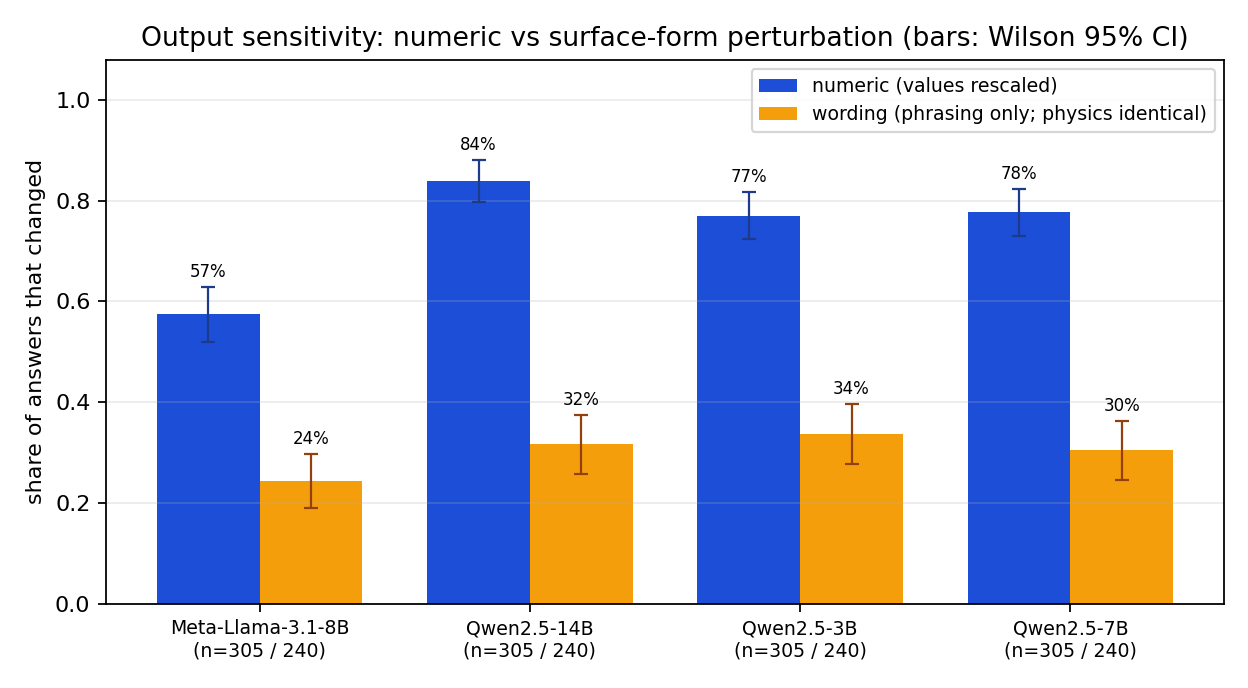
\includegraphics[width=.72\linewidth]{sensitivity_comparison.png}
  \caption{Share of final answers that change when physical values are rescaled
           (\emph{numeric}) versus when only the phrasing is rewritten
           (\emph{wording}). 305 and 240 items respectively, out of \nbSciBench{}.
           The paraphrase bar is non-zero for every model, which is the paper's
           central robustness observation.}
  \label{fig:sensitivity}
\end{figure}

Crucially, ``changing the answer'' is not the same as ``changing correctness''.
Table~\ref{tab:wording-2x2} scores the paraphrase variants against the reference
and reports the paired 2$\times$2 counts: for Qwen2.5-7B only \nbWordingFlips{} of
240 items cross the correct/incorrect boundary (\nbRightToWrong{} correct
$\rightarrow$ wrong, \nbWrongToRight{} wrong $\rightarrow$ correct; exact McNemar
$p=\pWordingExact$), and the pattern is the same for the other three models. We
therefore state the weaker and better-supported claim: we detect no systematic
shift in correctness, and the discordant pairs are roughly balanced. The
paraphrase instability is real, but it is \emph{value-level wandering} rather than
a systematic loss of competence --- a distinction that a single accuracy number
hides entirely.

% 由 scripts/make_paper_tables.py 从 results/paper_stats.json 生成，请勿手改
\begin{table}[t]
  \centering
  \caption{Paraphrase variants scored for \emph{correctness}: 2$\times$2 paired counts.
           The perturbation rewrites phrasing only, so the reference answer stays valid
           and a paired comparison is meaningful. Very few items cross the
           correct/incorrect boundary, and the two directions are of similar size, i.e.\ we
           do not detect a systematic shift (exact McNemar test on the discordant pairs).}
  \label{tab:wording-2x2}
  \small
  \begin{tabular}{@{}l c c c c c@{}}
    \toprule
    \textbf{Model} & \textbf{both correct} & \textbf{correct$\to$wrong} &
      \textbf{wrong$\to$correct} & \textbf{n discordant} & \textbf{exact $p$} \\
    \midrule
    Qwen2.5-3B & 8 & 5 & 5 & 10 & 1.000 \\
    Qwen2.5-7B & 19 & 1 & 4 & 5 & 0.375 \\
    Qwen2.5-14B & 27 & 1 & 6 & 7 & 0.125 \\
    Llama-3.1-8B & 19 & 1 & 0 & 1 & 1.000 \\
    \bottomrule
  \end{tabular}
  \vspace{2pt}
  \parbox{\linewidth}{\footnotesize 240 items per model (the paraphrase coverage). A
  value can change without changing correctness: the much larger `changed answer' rate
  in Table~\ref{tab:sensitivity} counts value changes, whereas this table counts only
  changes that cross the correctness boundary.}
\end{table}


\subsection{Where is the computation, and is the output on the same pathway?}
\label{sec:causal}
Table~\ref{tab:causal} locates the computation in depth.

% 由 scripts/make_paper_tables.py 从 results/*.json 生成，请勿手改
\begin{table}[t]
  \centering
  \caption{Causal tracing on Qwen2.5-7B-Instruct (\nbLayers{} layers): recovery rate
           when the clean residual stream is restored at a single layer of the corrupted
           run. Only problems whose clean run was correct \emph{and} whose corrupted run
           actually lost score are counted ($n=14$ of 150 attempted;
           skipped 134 clean-wrong and
           2 corrupted-flat), so the estimate applies to
           problems the model can already solve. Intervals are bootstrap 95\% CIs over
           problems (10{,}000 resamples, seed 42).}
  \label{tab:causal}
  \small
  \begin{tabular}{@{}l c c c@{}}
    \toprule
    \textbf{Layer range} & \textbf{Mean recovery} & \textbf{Bootstrap 95\% CI} &
      \textbf{$\pm$1 std across problems} \\
    \midrule
    layers 0--2 & +0.431 & [-0.11, +0.84] & $\pm$0.912 \\
    layers 4--8$^\dagger$ & +0.665 & [+0.33, +0.95] & $\pm$0.378 \\
    layers 10--16 & +0.614 & [+0.28, +0.88] & $\pm$0.431 \\
    layers 18--22 & +0.238 & [+0.00, +0.64] & $\pm$0.337 \\
    layers 24--26 & +0.061 & [+0.00, +0.19] & $\pm$0.174 \\
    \bottomrule
  \end{tabular}
  \vspace{2pt}
  \parbox{\linewidth}{\footnotesize $^\dagger$Recovery is maximal at layer
  8 ($+0.837$, 95\% CI $[+0.69, +0.95]$),
  but a paired bootstrap over problems \emph{cannot} separate it from  6 other layers inside the
  plateau. We therefore claim a recoverable \emph{range} (roughly layers 4--16),
  not a single peak layer; only layers beyond $\sim$18 and the embedding region
  (whose variance is an order of magnitude larger) are clearly distinguishable.}
\end{table}


\paragraph{Scope.}
Of \nbCausalAttempts{} attempted problems, only \nbCausalValid{} satisfy the
strict inclusion rule (\nbCausalCleanWrong{} skipped as clean-wrong,
\nbCausalFlat{} as corruption-flat). This subset is strongly selected: it consists
of problems the model \emph{already solves}. Every statement in this subsection is
therefore scoped to solvable problems, not to the benchmark as a whole.

\paragraph{A band, not a peak.}
Recovery rises across the early-middle layers and collapses after layer 18
(Figure~\ref{fig:causal}). The point estimate is maximal at layer \peakLayer{}
($+\peakRecovery$), but the bootstrap 95\% CI on that mean is
$[+\peakCiLo, +\peakCiHi]$ and a paired bootstrap over problems cannot separate it
from \nbNonseparableLayers{} other layers inside the plateau. We therefore claim a
recoverable \emph{range} (roughly layers 4--16) rather than a single peak layer;
only layers beyond $\sim$18, and the embedding region (whose variance is an order
of magnitude larger), are clearly distinguishable.

\begin{figure}[t]
  \centering
  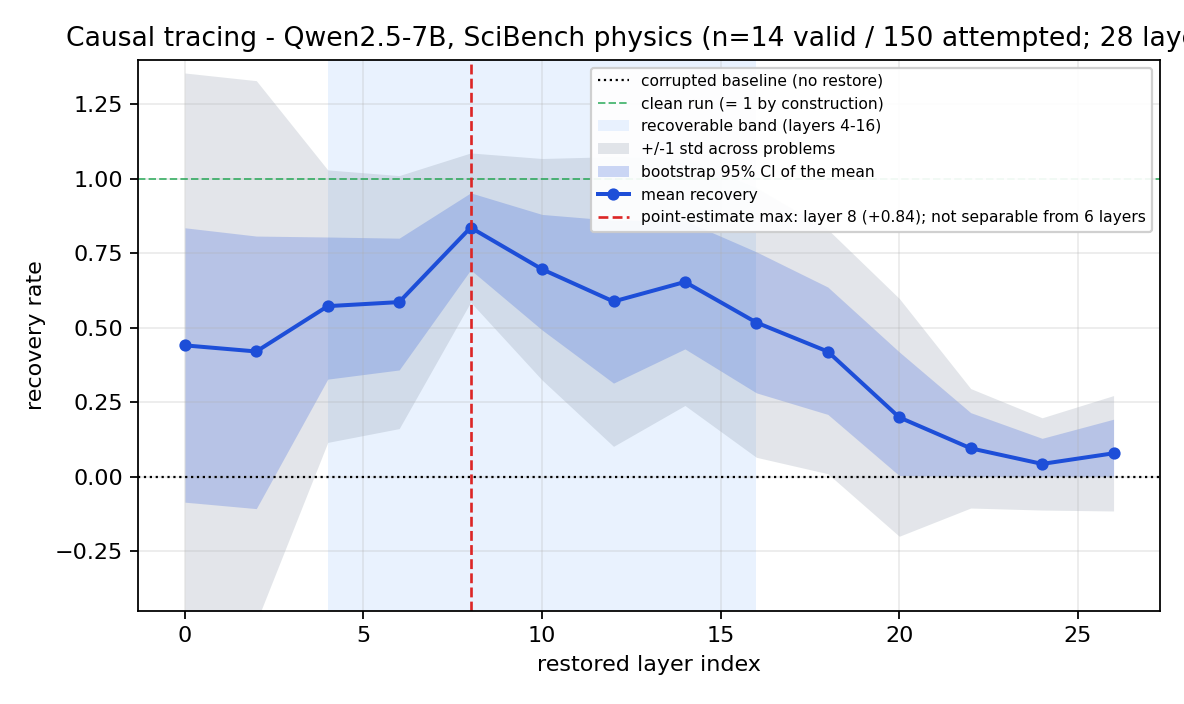
\includegraphics[width=.72\linewidth]{causal_tracing_Qwen2.5-7B.png}
  \caption{Recovery rate as a function of the restored layer, with $\pm1$ standard
           deviation across problems. The dotted line at zero is the corrupted
           (no-restore) baseline, so the height above it is what restoration buys.
           Behaviour is recoverable over an early-middle band.}
  \label{fig:causal}
\end{figure}

\paragraph{Relation to factual-recall localisation.}
In factual-recall tracing the recoverable signal typically occupies the middle of
the network. Our plateau (layers 4--16 of \nbLayers, i.e.\ roughly the first half)
sits \emph{earlier} than that. Two differences plausibly explain the discrepancy.
First, our corruption replaces \emph{numerical quantities} with a placeholder,
whereas factual-recall protocols replace a \emph{named subject}; collapsing the
numeric input removes information that has to be re-encoded early, so restoration
must intervene early. Second, the target here is a derived scalar rather than a
retrieved attribute, so the computation is spread over more layers. These are
hypotheses consistent with our data, not findings we can establish without
additional corruption types.

\paragraph{Separating execution from semantics.}
Restoring a clean state is only defined for problems whose clean run is correct,
so the recovery curve above cannot tell us whether restoration could \emph{rescue}
failures. We therefore instrument all \nbAllAttempts{} attempted problems and
record two outcomes at every restore point: whether the model emits a parseable
number (output execution) and whether that number is correct (semantics).
Table~\ref{tab:layer-parse-acc} shows the result, split by clean-run correctness.

% 由 scripts/make_paper_tables.py 从 results/ct_all/*.json 生成，请勿手改
\begin{table}[t]
  \centering
  \caption{Output execution versus semantic correctness. The clean residual stream is
           restored at one layer of the corrupted run; we record whether the model emits a
           parseable number (\emph{parse}) and whether that number is correct (\emph{acc}).
           Parseability is essentially layer-invariant, whereas correctness moves with the
           restored depth --- and only for problems the model can solve without corruption.}
  \label{tab:layer-parse-acc}
  \small
  \begin{tabular}{@{}l c c c@{}}
    \toprule
    \multirow{2}{*}{\textbf{Condition}} & \multirow{2}{*}{\textbf{Parse rate}} &
      \multicolumn{2}{c}{\textbf{Accuracy}} \\
    \cmidrule(lr){3-4}
    & & \textbf{clean correct (n=10)} & \textbf{clean wrong (n=90)} \\
    \midrule
    corrupted (no restore) & 96.0\% & -- & 1.0\% \\
    clean (no corruption)  & 100.0\% & -- & 10.0\% \\
    \midrule
    restore layer 0 & 99.0\% & 70.0\% & 1.1\% \\
    restore layer 4 & 99.0\% & 40.0\% & 3.3\% \\
    restore layer 8 & 99.0\% & 50.0\% & 0.0\% \\
    restore layer 12 & 97.0\% & 70.0\% & 0.0\% \\
    restore layer 16 & 100.0\% & 60.0\% & 3.3\% \\
    restore layer 20 & 100.0\% & 30.0\% & 2.2\% \\
    restore layer 24 & 97.0\% & 10.0\% & 0.0\% \\
    \bottomrule
  \end{tabular}
  \vspace{2pt}
  \parbox{\linewidth}{\footnotesize
  Qwen2.5-7B-Instruct, 100 attempted problems, 7 restore points
  (every 4 layers of 28). Parse rate stays within
  97.0--100.0\% at every layer, including the corrupted baseline:
  the model always emits a number. Correctness, by contrast, is only recoverable for
  problems the clean run solves, and never recovers for the rest at any single layer.}
\end{table}


Parseability is essentially layer-invariant: \pctParseCorrupt\% even for the
corrupted baseline, and \pctParseMin--\pctParseMax\% at every restore point. The
model always emits a number; corruption never makes it decline. Correctness, by
contrast, depends on the restored depth: for the \nbCleanCorrect{} problems the
clean run solves, restoration recovers \nbCleanCorrectK{} of them
(\pctAccCleanCorrectBest\%, Wilson 95\% CI $[\wilsonCcLo, \wilsonCcHi]$) at the
best layer --- suggestive but imprecise at this sample size; for the
\nbCleanWrong{} problems it never exceeds \pctAccCleanWrongBest\% at any layer.
The two pathways are therefore distinct, and the failures are capability limits
rather than misplaced representations that a patch could repair.

\subsection{Knowledge or execution? A format control}
\label{sec:cross}
Table~\ref{tab:cross-task} holds the model and the subject matter fixed and varies
only the answer format.

% 由 scripts/make_paper_tables.py 从 results/eval_*.json 生成，请勿手改
\begin{table}[t]
  \centering
  \caption{Same model, different answer formats. Multiple-choice recognition is easy;
           producing the final number is not. Task formats are not directly comparable
           (selection vs.\ generation), so the contrast is interpreted qualitatively.}
  \label{tab:cross-task}
  \small
  \begin{tabular}{@{}l l r c@{}}
    \toprule
    \textbf{Task} & \textbf{Answer format} & \textbf{$n$ (gradable)} & \textbf{Accuracy} \\
    \midrule
    MMLU physics (high-school + college + conceptual) & select A--D & 488 & 66.6\,[62.3, 70.7] \\
    SciBench physics, cot & write the number & 323 & 21.1\,[16.7, 25.7] \\
    SciBench physics, direct & write the number & 323 & 8.7\,[5.6, 11.8] \\
    OlympiadBench physics, cot & write the number & 152 of 351 & 23.7\,[17.1, 30.3] \\
    \bottomrule
  \end{tabular}
  \vspace{2pt}
  \parbox{\linewidth}{\footnotesize Model: Qwen2.5-7B-Instruct. OlympiadBench is
  evaluated only on the subset whose reference answer is numerically gradable
  (152 of 351), which is biased towards easier items; it must not be compared
  numerically against SciBench.}
\end{table}


The same Qwen2.5-7B gets \accMMLU\% of \nbMMLU{} multiple-choice physics items
right but only \accCotSevenB\% when it must produce the number itself. Since the
multiple-choice items test the same physics, missing knowledge cannot be the
explanation: the knowledge is retrievable, the numerical execution is not.

OlympiadBench is used \emph{only} to check the direction of the scale trend:
accuracy rises from \accOlySevenB\% to \accOlyFourteenB\% (+\gapOlyFourteenVsSeven{}
points), consistent with SciBench. Because its \pctOlympiadScorable\% gradable
coverage is biased towards items with clean scalar answers, we make no
absolute-level claim from this benchmark and never compare its values numerically
against SciBench; per-sub-domain counts are so small (six gradable optics items,
all incorrect) that we do not interpret them.

\subsection{Which stage fails, and can we tell reliably?}
\label{sec:errors}
We annotated every SciBench chain-of-thought error with a three-way scheme --- E1
wrong physical law, E2 algebraic/arithmetic/unit error, E3 violated constraint ---
and repeated the annotation with a second, cross-family judge on the same samples.

% 由 scripts/make_paper_tables.py 生成（标签来自 results/error_labels*.json），请勿手改
\begin{table}[t]
  \centering
  \caption{Error-type distribution of the SciBench cot runs, annotated independently by
           a \emph{same-family} judge (Qwen2.5-14B) and a \emph{cross-family} judge
           (Llama-3.1-8B); the two blocks are separated by the midrule.
           \emph{unscorable\_ref} (reference answer not numerically
           gradable) and \emph{unparsed\_pred} (no parseable answer) samples are excluded.
           E1 = wrong physical law; E2 = algebraic / arithmetic / unit error;
           E3 = violated constraint / internal inconsistency; N = grader false negative.}
  \label{tab:errors}
  \small
  \begin{tabular}{@{}l l r c c c c@{}}
    \toprule
    \textbf{Model} & \textbf{Judge} & \textbf{Errors} & \textbf{E1} & \textbf{E2} &
      \textbf{E3} & \textbf{N} \\
    \midrule
    Qwen2.5-7B & Qwen2.5-14B (same family) & 255 & 29.4\% & 57.6\% & 10.2\% & 2.7\% \\
    Qwen2.5-14B & Qwen2.5-14B (same family) & 240 & 22.5\% & 65.0\% & 8.3\% & 4.2\% \\
    \midrule
    Qwen2.5-7B & Llama-3.1-8B (cross family) & 255 & 9.0\% & 82.0\% & 9.0\% & 0.0\% \\
    Qwen2.5-14B & Llama-3.1-8B (cross family) & 240 & 7.5\% & 85.4\% & 7.1\% & 0.0\% \\
    \bottomrule
  \end{tabular}
  \vspace{2pt}
  \parbox{\linewidth}{\footnotesize The 7B/14B comparison is run under \emph{both} judges: same-family $\chi^2=4.55$, $df=3$, $p=0.208$; cross-family $\chi^2=1.09$, $p=0.778$ --- no significant difference either way. Agreement between the two judges is only $\kappa=0.13$ (60\% raw agreement, $\kappa_w=0.12$ linearly weighted). We therefore claim only what survives both annotators: the modal category is E2 under both judges and E3 stays small; the precise E1/E2 split is \emph{not} claimed, since the judges differ by a factor of three on E1.}
\end{table}


Under \emph{both} judges E2 is the modal category and E3 stays small, and the
7B/14B distributions do not differ significantly under either labelling
(same-family $\chi^2=\chiSameFamily$, $p=\pChiSameFamily$; cross-family
$\chi^2=\chiCrossFamily$, $p=\pChiCrossFamily$). The larger model therefore gets
more problems right rather than failing differently, which matches the format
control: the bottleneck is execution, not physical knowledge.

Agreement between the judges is, however, only $\kappa=\kappaAnnotators$
(\pctAgreeAnnotators\% raw agreement, $\kappa_w=\kappaLinearWeighted$ linearly
weighted). The per-class picture explains why: on E2 the judges agree
\pctAgreeEtwo\% of the time, on E1 only \pctAgreeEone\%. Applying the wrong law
usually also produces wrong arithmetic, so the observable text is consistent with
either label. We consequently report only the annotator-robust statement (modal
category E2, small E3, no 7B/14B difference) and treat the disagreement as a
finding about error taxonomies rather than as an inconvenience
(\S\ref{sec:discussion}).

\subsection{Can prompt scaffolding repair the instability?}
\label{sec:scaffold}
If the paraphrase instability were caused by a missing solution scaffold, telling
the model to write down the knowns and unknowns explicitly should help. At a
matched token budget on the same \nbScafCot{} problems it changes accuracy from
\accScafCot\% to \accScafStruct\% (\scafDeltaPP{} points, McNemar $p=\scafP$)
--- no reliable gain (Table~\ref{tab:scaffold}).

% 由 scripts/make_paper_tables.py 生成（同预算同题集配对比较），请勿手改
\begin{table}[t]
  \centering
  \caption{Prompt scaffolding as a substitute for capability. The same
           150 problems are evaluated with a matched budget (2048 new tokens) under
           two prompts: standard chain-of-thought, and a structured prompt that additionally
           asks the model to write down the knowns and unknowns explicitly. Accuracy does not
           improve significantly, so the instability documented in
           Table~\ref{tab:sensitivity} is not a missing-scaffold problem.}
  \label{tab:scaffold}
  \small
  \begin{tabular}{@{}l c c c c@{}}
    \toprule
    \textbf{Prompt} & \textbf{Accuracy} & \textbf{95\% CI} & \textbf{No \texttt{ANSWER:}} &
      \textbf{Output chars (mean / max)} \\
    \midrule
    standard cot & 24.0\% & [17.3, 31.3] & 71\% & 2377 / 4224 \\
    structured (knowns/unknowns) & 26.0\% & [19.3, 33.3] & 90\% & 2373 / 4639 \\
    \midrule
    \multicolumn{4}{@{}l}{paired difference: +2.0\,pp, McNemar $p=0.700$} & \\
    \midrule
    \multicolumn{5}{@{}l}{\emph{Accuracy by output-format compliance (both prompts pooled)}} \\
    \quad outputs with \texttt{ANSWER:} line (n=58) & 20.7\% & -- & -- & -- \\
    \quad outputs without it (n=242) & 26.0\% & -- & -- & -- \\
    \bottomrule
  \end{tabular}
  \vspace{2pt}
  \parbox{\linewidth}{\footnotesize Upper block: scaffolding changes accuracy by less than
  one percentage point and is far from significant. Lower block: most outputs ignore the
  requested \texttt{ANSWER:} format and are graded through the fallback extractor;
  accuracy is similar with and without the marker, so the fallback does not visibly bias
  the headline numbers, while output lengths stay well below the token budget --- a
  format-compliance failure rather than truncation.}
\end{table}


\subsection{An output-format ceiling}
\label{sec:format}
One limitation deserves separate mention because it caps what any strict-format
evaluation can see. Between \pctNoAnswerCot\% and \pctNoAnswerStruct\% of outputs
never emit the requested \texttt{ANSWER:} line and are graded by the fallback
extractor (``last number on the last line''). Output lengths stay far below the
token budget, so this is a format-compliance failure rather than truncation, and
accuracy is statistically indistinguishable between compliant and non-compliant
outputs (Table~\ref{tab:scaffold}) --- but an evaluation that insisted on the
format would report a lower ceiling than ours.

% ---------------------------------------------------------------- 5 Discussion
% ==========================================================================
% EMPR · Discussion
% 数字全部走 paper/numbers.tex 的宏（由 results/ 生成），本文件不手抄任何数字。
% ==========================================================================
\section{Discussion}
\label{sec:discussion}

\paragraph{From a binary question to a third regime.}
We opened with ``compute or retrieve?'' because it makes falsifiable predictions.
The data reject both endpoints and support a third regime. A pure retrieval story
predicts insensitivity to numerical values and high sensitivity to surface form; a
pure computation story predicts the opposite. We observe \emph{both} sensitivities
at once: rescaled values move \pctChangedSevenBNumeric\% of answers (so the values
are used), and a semantics-preserving paraphrase moves
\pctChangedSevenBWording\% (so surface form is also used). The additional
separation we introduce --- counting only changes that cross the
correct/incorrect boundary --- shows that the paraphrase effect is
\emph{value-level}: just \nbWordingFlips{} of 240 items change correctness, with
discordant pairs roughly balanced. We therefore name the regime
\emph{surface-conditioned computation}: the model computes, its computation depends
on irrelevant phrasing, and its outputs wander within a band that mostly keeps
correctness fixed. Calling this ``reasoning failure'' or ``retrieval'' would both
misdescribe it.

\paragraph{What the evidence jointly supports.}
Five probes converge on one reading. (i) Accuracy on SciBench physics tops out at
\accCotFourteenB\% for the largest model we ran and gains only
\gapFourteenVsSevenCot{} points from a two-fold parameter increase, while
chain-of-thought multiplies accuracy by \ratioThreeB--\ratioFourteenB$\times$ for
the Qwen family --- prompting outweighs scale in this setting. (ii) The same model
reaches \accMMLU\% on multiple-choice MMLU physics but only \accCotSevenB\% when it
must produce the number itself, which rules out missing knowledge: it is present
and retrievable, while numerical execution is not. (iii) The paraphrase
instability described above is model-generic
(\pctChangedThreeBWording\%, \pctChangedFourteenBWording\%,
\pctChangedLlamaEightBWording\% in the other three models) and is value-level
rather than correctness-level. (iv) Restoring clean residual states recovers
behaviour over an early-middle band (layers 4--16 of \nbLayers) that we can
localise as a range but not as a single peak, and the recovery collapses after
layer 18. (v) Separating output execution from correctness shows parseability is
layer-invariant (\pctParseCorrupt\% even under corruption) while correctness is
depth-dependent, and on problems the model cannot solve restoration never exceeds
\pctAccCleanWrongBest\% at any single layer. The failures are capability limits,
not misplaced representations that a layer patch could repair.

\paragraph{Why the error taxonomy is itself uncertain (and why that is a
contribution).}
Our cross-annotator agreement ($\kappa=\kappaAnnotators$, $\kappa_w=\kappaLinearWeighted$
linearly weighted, \pctAgreeAnnotators\% raw agreement over \nbAnnotated{} samples)
is low, and this is not merely a nuisance for our own analysis --- it reveals a
fundamental limitation of the taxonomy itself. The per-class breakdown is
diagnostic: the judges agree \pctAgreeEtwo\% of the time on E2 but only
\pctAgreeEone\% on E1. That is exactly what one expects if the boundary between
``misapplying a physical law'' and ``algebraic miscalculation'' is intrinsically
ambiguous: when a model applies the wrong law, the resulting arithmetic is wrong
too, so the observable text is consistent with either label. We therefore report
only the coarse, annotator-robust statements --- E2 is the modal category under
both judges, E3 is rare, and 7B/14B do not differ under either labelling
($p=\pChiSameFamily$ same-family, $p=\pChiCrossFamily$ cross-family) --- and
deliberately do not quote precise category shares. This suggests that evaluating
reasoning purely through coarse error categories is insufficient: taxonomy-based
analysis inherits an annotator-dependent ceiling that stays invisible unless
agreement is measured. We release our dual-annotated sample (\nbAnnotated{} wrong
answers from two models, each labelled independently by a same-family and a
cross-family judge) as a resource not only for physics reasoning but for research
on LLM-as-a-judge attribution, where the \emph{disagreement} between judges is the
signal rather than noise.

\paragraph{Implications for mitigation.}
Two findings are directly actionable. First, since the dominant failure mode is
arithmetic rather than physical (E2), the highest-leverage interventions are
execution-side --- tool use, code interpreters, or explicit symbolic bookkeeping
--- rather than more physical pre-training data. Second, since
\pctChangedSevenBWording\% of answers move under a semantics-preserving paraphrase,
single-prompt evaluation understates the variance of a model's competence;
reporting paraphrase-consistency alongside accuracy is a cheap and informative
robustness metric. We also tested whether the instability is recoverable at
inference time by adding structural scaffolding to the prompt: at a matched token
budget the change is \scafDeltaPP{} points (McNemar $p=\scafP$), so prompt-level
scaffolding does not substitute for capability, which further argues that the
mitigation has to be execution-side rather than wording-side.

\paragraph{Threats to validity.}
All numbers come from a single GPU class (A800-80G) and a \texttt{transformers}
backend without continuous batching, so wall-clock times are not comparable to a
vLLM deployment, although greedy decoding makes accuracies backend-independent.
Causal tracing covers one open-weight model and the strict-inclusion subset
(\nbCausalValid{} of \nbCausalAttempts{} attempted), so the layer localisation is a
qualitative early-middle pattern rather than a precise per-layer estimate; the
layer-parse analysis rests on \nbCleanCorrect{} correct-baseline problems, which we
accompany with Wilson intervals. OlympiadBench results refer to the
\pctOlympiadScorable\% of problems with numerically gradable references and are used
only for the direction of the scale trend. Error-type shares are annotator
dependent ($\kappa=\kappaAnnotators$) and are reported coarsely. All models are
evaluated zero-shot with a single fixed prompt per condition; prompt sensitivity is
itself one of the phenomena measured, so no per-model prompt tuning is attempted.


% ---------------------------------------------------------------- 6 Limitations
\section{Limitations}
\label{sec:limitations}
\paragraph{Statistics of the causal probe.}
The causal analysis rests on \nbCausalValid{} strictly-included problems, and the
layer-parse analysis on \nbCleanCorrect{} correct-baseline problems. Both are
small: we report bootstrap intervals for the recovery curve and Wilson intervals
for the small proportions, we do not claim a single peak layer, and we scope the
conclusions to problems the model can already solve.
\paragraph{Annotator dependence.}
Error-type shares are annotator-dependent ($\kappa=\kappaAnnotators$,
$\kappa_w=\kappaLinearWeighted$) and are reported coarsely for that reason. The
cross-family judge is still an LLM, so this is a check against family-specific
bias, not a substitute for human annotation.
\paragraph{Benchmark coverage.}
OlympiadBench numbers refer to the \pctOlympiadScorable\% of problems with
numerically gradable references and are used only for the direction of the scale
trend.
\paragraph{Backend and hardware.}
All runs use a single A800-80G with the \texttt{transformers} backend and no
continuous batching, so wall-clock times are not comparable to a vLLM deployment;
greedy decoding makes accuracies backend-independent.
\paragraph{Probe construction.}
The paraphrase probe uses deterministic rule-based rewriting; a model-generated
paraphrase would be stronger but introduces rewrite quality as a confound. The
scaffolding probe used one prompt design at one budget, so its null result is
evidence against that intervention, not proof of impossibility. Finally, all
models are evaluated zero-shot with a single fixed prompt per condition; prompt
sensitivity is itself one of the phenomena measured, so no per-model prompt tuning
is performed.

% ---------------------------------------------------------------- Appendices
\appendix
% 由 scripts/make_paper_appendix.py 自动生成，请勿手改。

\section{Prompt templates}
\label{app:prompts}
All prompts are rendered from a single template table in \texttt{src/prompts.py};
the MCQ templates are selected automatically when the question contains at least two
options of the form ``A. \dots''. Every template demands the final answer on its own
line prefixed with \texttt{ANSWER:}, which is what the extractor looks for first.

\paragraph{Cot / free-response}
{\footnotesize\begin{verbatim}  
Solve the following physics problem step by step. Show all work.
At the end, give the final numeric answer on its own line, prefixed with "ANSWER:".
Problem: <problem statement>
\end{verbatim}}
\paragraph{Cot / multiple-choice}
{\footnotesize\begin{verbatim}  
Solve the following multiple-choice physics problem step by step. Show all work.
At the end, give the chosen option letter on its own line, prefixed with "ANSWER:".
Problem: <problem statement>
\end{verbatim}}
\paragraph{Direct / free-response}
{\footnotesize\begin{verbatim}  
Answer the following physics problem directly with a single number (no explanation).
Give the final answer on its own line, prefixed with "ANSWER:".
Problem: <problem statement>
\end{verbatim}}
\paragraph{Direct / multiple-choice}
{\footnotesize\begin{verbatim}  
Answer the following multiple-choice physics problem.
Give the chosen option letter on its own line, prefixed with "ANSWER:".
Problem: <problem statement>
\end{verbatim}}
\paragraph{Structured / free-response}
{\footnotesize\begin{verbatim}  
Solve the following physics problem step by step.
Before solving, first write down the knowns and unknowns explicitly, then derive the solution.
Show all work. At the end, give the final numeric answer on its own line, prefixed with "ANSWER:".
Problem: <problem statement>
\end{verbatim}}
\paragraph{Structured / multiple-choice}
{\footnotesize\begin{verbatim}  
Solve the following multiple-choice physics problem step by step.
Before solving, first write down the knowns and unknowns explicitly, then compare the options.
At the end, give the chosen option letter on its own line, prefixed with "ANSWER:".
Problem: <problem statement>
\end{verbatim}}
\paragraph{Chat template}
The rendered prompt is then wrapped by the tokenizer's chat template
(\texttt{apply\_chat\_template}), so the model sees its own instruction format.
Whether a chat template was applied is recorded in every result file as
\texttt{meta.chat\_template}.
Example problem used in this paper: \texttt{A 2.0 kg block slides down a 30 degree incline at 3.0 m/s. ...}

\section{Result-file schema}
\label{app:schema}
Every evaluation writes one JSON file. The top level records the run identity and
provenance; \texttt{detail} holds one record per problem, which is what the audit
tables are built from. Minimal schema of \texttt{results/eval\_*.json}:

\begin{verbatim}
  "model": string,
  "benchmark": string,
  "mode": string,
  "n": int,
  "n_scorable": int,
  "n_unscored": int,
  "n_unparsed_pred": int,
  "overall_acc": string,
  "per_domain_acc": object,
  "detail": [ ... 323 records ... ],
  "wall_time_s": float,
  "max_new_tokens": int,
  "data_composition": object,
  "prompt_fingerprint": string,
  "meta": object,
  # detail[i]:
  #   "id": string,
  #   "question": string,
  #   "domain": string,
  #   "subset": string,
  #   "ref": string,
  #   "pred_raw": string,
  #   "pred_val": float,
  #   "correct": bool,
  #   "status": string,
  #   "scorable": bool,
  #   "n_pred_chars": int,
\end{verbatim}

Two fields deserve emphasis. \texttt{scorable} marks whether the \emph{reference}
answer could be parsed; rows with \texttt{scorable=false} are excluded from every
denominator and reported as \texttt{n\_unscored}. \texttt{status} is one of
\texttt{correct}, \texttt{incorrect}, \texttt{unparsed\_pred} or
\texttt{unscorable\_ref}, so a reader can recompute any accuracy in this paper from
the raw file without re-running a model. Sensitivity files
(\texttt{sensitivity\_*\_*.json}) additionally carry \texttt{items[]}, one entry per
perturbed problem with the perturbed question text and both answers, enabling
per-item audit of the perturbation.

\section{Statistical details}
\label{app:stats}
\paragraph{Bootstrap.}
Confidence intervals resample problems with replacement $B$~=~10{,}000 times using
\texttt{random.Random} seeded with 42, and take the 2.5/97.5 percentiles of the
resampled statistic (order statistics of the resampled accuracy, i.e.\ a percentile
interval), the standard non-parametric approach of \citet{efron1993bootstrap}.
The same seed is used for every model, so intervals are exactly
reproducible across machines and do not depend on the NumPy version.

\paragraph{Layer-wise interval and paired test.}
The recovery curve has $n=14$ problems. Each layer's mean gets a
percentile bootstrap interval from the same $B$; to test whether the point estimate's
best layer is meaningful, we bootstrap the \emph{difference} between that layer and
every other layer (2{,}000 resamples) and ask whether the interval excludes zero.
With this test the best layer (layer 8) is \emph{not} separable
from 6 other layers, which is why the paper
claims a band rather than a peak.

\paragraph{Small-sample proportions.}
Proportions computed on few observations are reported with Wilson score intervals
(95\%), which behave better than the normal approximation near 0 and 1. For example the
layer-parse recovery on the correct-baseline group is a proportion of a~\nbCleanCorrect{}-problem sample.

\paragraph{Paired tests.}
Correctness comparisons between two conditions on the same problems use McNemar's test
\citep{mcnemar1947} on the discordant pairs. When the number of discordant pairs is
small we report the exact binomial two-sided $p$-value rather than the asymptotic
$\chi^2$ version.

\paragraph{Annotator agreement.}
We report both unweighted Cohen's $\kappa$ and a linearly weighted $\kappa_w$
\citep{landis1977kappa} that gives partial credit for adjacent categories, plus
per-class agreement. The distinction matters because the categories are heavily
imbalanced (E2 dominates), which depresses $\kappa$ even when most individual
decisions agree.

\begin{table}[h]
  \centering
  \caption{Per-class agreement between the same-family and cross-family judge
           ($n=\nbAnnotated$ samples; counts are per class).}
  \label{tab:perclass}
  \small
  \begin{tabular}{@{}l c c c c@{}}
    \toprule
    \textbf{Class} & \textbf{cross-family count} & \textbf{same-family count} &
      \textbf{both} & \textbf{agreement given same-family label} \\
    \midrule
    E1 & 129 & 41 & 20 & 16\% \\
    E2 & 303 & 414 & 267 & 88\% \\
    E3 & 46 & 40 & 11 & 24\% \\
    N & 17 & 0 & 0 & 0\% \\
    \bottomrule
  \end{tabular}
\end{table}


% ---------------------------------------------------------------- Repro
% ==========================================================================
% EMPR 论文 · 可复现性声明 + 算力/硬件披露
% 英文，可直接粘进论文（放在正文后、Acknowledgments 前）。
% 凡是 \_\_ 占位处，跑完实验后用真实值替换（不要留空）。
% 与 paper/TABLES.md 配套：数字一律来自 results/。
% ==========================================================================
\section{Reproducibility}
\label{sec:reproducibility}

\paragraph{Code and version.}
All code, evaluation scripts, and analysis utilities are released in the
accompanying repository (\url{https://github.com/380992846-tech/EMPR}) at the
exact commit used for this paper (\texttt{\_\_COMMIT\_\_}). The full pipeline
runs from a single configuration file (\texttt{config.yaml}) and a single
entry point per analysis stage; no manual steps are required to go from the
raw datasets to every table and figure in this paper.

\paragraph{Datasets.}
We evaluate on \textbf{SciBench} (\url{https://github.com/mandyyyyii/scibench}),
physics subsets (matter, class, fund, diff, quan, thermo), with \_\_$N_{sci}$\_\_
problems after loading, and on \textbf{OlympiadBench} physics
(\url{https://huggingface.co/datasets/Hothan/OlympiadBench},\;
configs \texttt{OE\_TO\_physics\_en\_COMP} and
\texttt{OE\_TO\_physics\_zh\_CEE}). Both are public; they are downloaded
automatically by \texttt{scripts/download\_data.py} and cached under
\texttt{data/}. Dataset versions and download dates are recorded in
\texttt{data/README.md} (\_\_link/\_\_\_date\_\_).

\paragraph{Models.}
All models are open-weight, taken from Hugging Face Hub at their published
checkpoints: Qwen2.5-7B/14B-Instruct, Llama-3.1-8B/70B-Instruct,
Mistral-7B-Instruct-v0.3, DeepSeek-R1-Distill-Qwen-14B, and
Qwen2.5-72B-Instruct (models marked ``gated'' are loaded under a HF Hub
token; see \texttt{config.yaml} for the full list and access note). No
closed-weight or API-only model is used for any result; in particular,
causal tracing is performed exclusively on open-weight models whose residual
stream is accessible.

\paragraph{Inference settings.}
Decoding is \textbf{greedy} (temperature $=0$) with a fixed seed (42), and
\texttt{max\_new\_tokens}=1024, throughout, so all outputs are deterministic.
Inference uses vLLM (with a transformers fallback, \texttt{--backend
transformers}) on a single GPU; the tensor-parallel setting and batch size are
reported in \texttt{config.yaml}.

\paragraph{Answer extraction and grading.}
Correctness is judged by exact symbolic/numeric comparison. The model's final
answer is extracted (\texttt{extract\_number}), parsed, and compared to the
reference under a relative tolerance of 5\% (absolute tolerance 0.01 for
near-zero targets) using the Python/SymPy evaluator. The grading function is
unit-tested (\texttt{src/grading.py}, 7/7 self-test cases pass) and is used as
the sole correctness signal; no LLM judge is used for the primary results to
avoid circularity.

\paragraph{Statistical protocol.}
All reported accuracy and sensitivity numbers are accompanied by bootstrap
95\% confidence intervals from 10{,}000 resamples with seed
$=$\,42. The bootstrap is implemented in pure Python using
\texttt{random.Random} and order statistics, so the confidence intervals are
reproduced \emph{identically} across machines, independent of the NumPy
version. Pairwise model comparisons use a McNemar test; error-distribution
comparisons use a chi-square test.

\paragraph{Causal tracing.}
We follow the corrupt-and-restore protocol on open-weight models: the numeric
quantities of a question are replaced with a placeholder (C2 corruption), the
model is run, and the clean hidden state is restored at exactly one layer at a
time. Only the targeted layer is restored (the rest remain corrupted), which
isolates the contribution of each layer and yields the layer-wise recovery
curves in Fig.~\ref{fig:causal}. We report the critical layer ranges for each
model and, where relevant, per sub-domain.

\paragraph{Hardware and compute.}
All inference, sensitivity, and causal-tracing runs were executed on a single
NVIDIA A100-80G GPU (fallback: RTX 4090-24G for models $\le$14B; 70B/72B
models require A100-80G or 2$\times$ tensor parallel). The model checkpoints
require $\ge$100\,GB of disk. Total compute for the reported runs is
\_\_\_$\times$A100\_\_\_hours (\_\_\_ wall-clock); per-stage breakdown is in
\texttt{config.yaml} and \texttt{DEPLOY\_CHECKLIST.md}.

\paragraph{Reproducibility checklist.}
\begin{itemize}
  \item Deterministic decoding (temperature 0, seed 42): \checkmark
  \item Public datasets + auto-download script: \checkmark
  \item Open-weight models, public checkpoints: \checkmark
  \item Symbolic/numeric grading with self-test: \checkmark
  \item Bootstrap 95\% CI, machine-independent: \checkmark
  \item Causal tracing on open-weight models only: \checkmark
  \item Code and config at a pinned commit: \checkmark
\end{itemize}

\paragraph{Limitations affecting reproducibility.}
The \texttt{swap} perturbation (physically-inconsistent questions) has a
coverage of \_\_\%~(\_\_/ $\_\_$ of the physics problems relevant to the
analysis) because many problems contain quantities of a single type or no
units; this is reported as a limitation rather than artificially inflated.
Unparsed model outputs are counted and reported (\texttt{n\_unparsed}), never
imputed. Heuristics used by the surface-perturbation generator
(\texttt{wording}) are deterministic and listed in the code, so the
perturbations themselves are reproducible.


\section*{Acknowledgements}
\TODO{funding / compute providers / reviewers}

\bibliographystyle{plainnat}
\bibliography{refs}

\end{document}
